\documentclass[a4paper,cs4size,adobefonts,fancyhdr]{ctexart}[2005/11/25]
\usepackage[
     left=2.7cm,
     right=2.7cm,
     top=3.5cm,
     bottom=2.6cm]{geometry}
\usepackage{fancyhdr}
\pagestyle{fancy}

\fancyhf{}
\fancyhead[EC,OC]{\zihao{-5}北京化工大学毕业设计(论文)中期检查报告}
\fancyfoot[C]{\thepage}
\renewcommand{\headrulewidth}{0pt}
\renewcommand{\footrulewidth}{0pt}     

\usepackage[numbers,sort&compress]{natbib}   % bibtex 自然序号

\CTEXsetup[format+=\zihao{-3}]{chapter}
\CTEXsetup[format+=\zihao{-3}]{section}
\CTEXsetup[format+=\zihao{-4}]{subsection}
\CTEXsetup[format+=\zihao{-4}]{subsubsection}
%-------------------------------------------------------


\newcommand{\upcite}[1]{\textsuperscript{\textsuperscript{\cite{#1}}}}

\newCJKfontfamily[shusong]\shusong{方正书宋_GBK}
\newCJKfontfamily[biaosong]\biaosong{方正小标宋_GBK}


\usepackage{longtable}
\usepackage{booktabs}
\usepackage[version=3]{mhchem}
\usepackage{tikz}
\usepackage{sistyle}
\usepackage{graphicx}
\usepackage{amsmath}
\usepackage{wasysym}
\usepackage{floatflt}
%\usepackage{caption2}
\usepackage{amsfonts}
\usepackage{mdwlist}
\usepackage{tabularx}
\usepackage{subfig}  %子浮动体
\usepackage{caption}
\usepackage{floatrow}
\floatsetup[table]{style=plaintop} 
\numberwithin{equation}{section} %公式章节编号
%\usepackage{times}
%\usepackage{mathtime}
%\usepackage{minionpro}
%\CTEXsetup[name={,},number={\arabic{chapter}},format={\Large\bfseries}]{chapter}
% \CTEXsetup[format={\Large\bfseries}]{section}
%引用上标定义
\makeatletter
\def\@cite#1#2{\textsuperscript{[{#1\if@tempswa , #2\fi}]}}
\newcommand*{\rom}[1]{\expandafter\@slowromancap\romannumeral #1@}
\newcommand{\dif}{\mathrm{d}}
\newtheorem{Definition}{定义}[section]
\newtheorem{Theorem}[Definition]{定理}
\makeatother
\title{\heiti 微生物土壤运移模型的求解及仿真软件编制\\中期检查报告}
\author{\kaishu 陆秋文 \\ \kaishu 北京化工大学生命科学与技术学院}
\date{}
\begin{document}
\begin{titlepage}
\thispagestyle{empty}
\newcommand{\HRule}{\rule{\linewidth}{0.5mm}} % Defines a new command for the horizontal lines, change thickness here

\center % Center everything on the page
 
%----------------------------------------------------------------------------------------
%	HEADING SECTIONS
%----------------------------------------------------------------------------------------

% \textsc{\Large 北京化工大学}\\[1.5cm] % Name of your university/college
\vspace*{1.2cm}
\textsc{\zihao{-3} 北京化工大学本科毕业设计(论文)}\\[2.8cm] % Major heading such as course name
% \textsc{\large Minor Heading}\\[0.5cm] % Minor heading such as course title

%----------------------------------------------------------------------------------------
%	TITLE SECTION
%----------------------------------------------------------------------------------------

\vspace*{1.2cm}
{\heiti \zihao{2}微生物土壤运移模型的求解及仿真软件编制 \biaosong\zihao{2} \\ [0.8cm]外文文献翻译}\\[1cm] % Title of your document
\vspace*{1.2cm}
 
%----------------------------------------------------------------------------------------
%	AUTHOR SECTION
%----------------------------------------------------------------------------------------

% \begin{minipage}{0.4\textwidth}
% \begin{flushleft} \large
% \emph{作者:}\\
% John \textsc{Smith} % Your name
% \end{flushleft}
% \end{minipage}
% ~
% \begin{minipage}{0.4\textwidth}
% \begin{flushright} \large
% \emph{Supervisor:} \\
% Dr. James \textsc{Smith} % Supervisor's Name
% \end{flushright}
% \end{minipage}\\[4cm]
{\kaishu\large
陆秋文\\
北京化工大学生命科学与技术学院\\[0.5cm]}
指导教师\\
{\large\kaishu 周\quad 延}
% If you don't want a supervisor, uncomment the two lines below and remove the section above
%\Large \emph{Author:}\\
%John \textsc{Smith}\\[3cm] % Your name

%----------------------------------------------------------------------------------------
%	DATE SECTION
%----------------------------------------------------------------------------------------
\vfill
% {\large 北京化工大学}\\
{\large 二〇一三年六月三日}\\[0.5cm] % Date, change the \today to a set date if you want to be precise

%----------------------------------------------------------------------------------------
%	LOGO SECTION
%----------------------------------------------------------------------------------------

%\includegraphics{Logo}\\[1cm] % Include a department/university logo - this will require the graphicx package
 
%----------------------------------------------------------------------------------------

 % Fill the rest of the page with whitespace
\end{titlepage}

% \maketitle
\setlength{\baselineskip}{22pt}
\section{问题的背景}
在环境工程领域,我们需要对受污染的土壤进行治理。一个比较好的方法就是生物原位修复,即将分离的到的或基因工程合成的细菌或营养物质注入土壤,使其运移到受污染处并大量繁殖,分解有毒物质,达到治理目的。这样,我们需要对土壤中微生物的运动规律进行研究。\par
在解决传染病、垃圾处理、污水灌溉处理等问题上,人们逐渐认识到了微生物在这些介质中运动是有一定规律的,并有一些学者在这些领域上对微生物的运动规律进行了研究。随着研究的深入和微生物在提高石油开采量、放射性物质和有机污染物的携带运移、提高冶炼率等问题中的应用,更加需要对微生物运动规律的了解,而且要求越来越精确。这样,对微生物运动规律的研究就显得格外有意义。\par
微生物在土壤中的运移过程看似简单,实际很复杂。其运移机理包括生长、吸附、解吸、沉积(过滤、布朗扩散、截流、沉降)、腐解、钝化、滞留等过程,确定微生物运移速率、时间、分布范围,最大限度地提高细菌降解作用,减少细菌本身的再污染,有必要对微生物在土壤中运移及其影响因素进行定量研究,建立数学模型。
\section{问题的数学模型}
为了对微生物运动位移进行定量研究,首先应当清楚影响其运动的原因。这个原因有两个方面,一为土壤地下水环境造成的影响,另外一个是微生物自身的因素。
\subsection{影响微生物运移规律的因素}
微生物在土壤多孔介质中的迁移受到各种非生物和生物因素的影响。这些因素可概括为两个主要方面,即水文地质因素和微生物因素。其中水文地质因素包括多孔介质的结构、质地、有机质含量、氧化膜以及地下水水流速度、溶液化学成分、溶液pH值、离子强度等;微生物因素包括细胞的生理状态、细胞的生长与衰亡、细胞的趋磁性、细胞的吸附过程、过滤效应等。除上述因子控制细菌迁移以外,各因子互相影响也很复杂,而且微生物本身是活体,常被称为“活胶体”,受环境影响较大。以上这些复杂因素就增加了微生物迁移研究的难度。\par
微生物方面的因素对其运移规律也有着重要的影响,包括微生物吸附、微生物生理状态、微生物运动性、趋向性等。
\subsection{数学模型的建立}
为了建立微生物在饱和地下环境中迁移过程的数学模型,在对微生物迁移过程研究中,作如下基本假定:
\begin{enumerate}\setlength{\itemsep}{0em}
\item 土壤是一个均质体; 
\item 水流是稳定的; 
\item 土壤孔隙率是一定的; 
\item 微生物细胞在液相中均匀悬浮; 
\end{enumerate}\par
根据资料,我们看到液相微生物的质量守恒方程,表示为:
\begin{equation}\label{equ:yexiangshouheng}
\dfrac{\partial(\theta S_w C_w)}{\partial t}
=-\nabla(\theta S_w C_w v_w)+\nabla[\theta S_wD_w\nabla v_w]+I+B_w
\end{equation}
式中,
	\begin{quote}
	\begin{description}\setlength{\itemsep}{0em}
	\item[$\theta$]为介质的孔隙度;
	\item[$S_w$]为含水饱和度;
	\item[$C_w$]为液相中微生物的浓度,\SI{}{mol/L^3};
	\item[$V_w$]为液相的总流动速度,\SI{}{L/T};
	\item[$D_w$]液相微生物的物理弥散系数,\SI{}{L^2/T};
	\item[$I$]为单位体积土壤中微生物在液相固相之间的传质速率,\SI{}{mol/(TL^3)};
	\item[$B_w$]为微生物生长的生物反应速率,\SI{}{mol/(TL^3)}
	\end{description}
	\end{quote}\par
式~\ref{equ:yexiangshouheng}~左侧表示微生物的累积,右侧第一项为对流项,第二项为水动力弥散项,第三项为相间传质项,第四项为生物反应项。\par
考虑一个方向,微生物的迁移方程简化为:
	\begin{equation}\label{qianyif}
	\dfrac{\partial C}{\partial t}=D\dfrac{\partial^2 C}{\partial x^2}-\nu\dfrac{\partial C}{\partial x}-k_{att}\theta C+k_{det}\rho S+\sigma C
	\end{equation}
式中,
	\begin{quote}
	\begin{description}\setlength{\itemsep}{0em}
%	\item[$\theta$]为介质体积含水率,对于饱和土壤,则是介质有效孔隙度;
	\item[$C$]为微生物在水相中的浓度,\SI{}{mg/m^3};
	\item[$S$]为微生物在固体表面可逆吸附的浓度,\SI{}{mg/g};
	\item[$\rho$]为土壤的容重,\SI{}{g/m^3};
	\item[$D$]为水动力弥散系数,\SI{}{m^2/s};
	\item[$v$]为流速,\SI{}{m/s}
	\item[$k_{att}$]为可逆吸附常数,\SI{}{s^{-1}}
	\item[$k_{det}$]为可逆解析常数,\SI{}{s^{-1}}
	\item[$\sigma$]为微生物比生长速率,\SI{}{s^{-1}}
	\end{description}
	\end{quote}\par
其中,流速只考虑孔隙流速,孔隙流速可以表示为:
\begin{equation}
	v=\dfrac{Q}{A\theta}
\end{equation}
式中,
	\begin{quote}
	\begin{description}\setlength{\itemsep}{0em}
	\item[$Q$]表示测定微生物穿透曲线的控制流量,\SI{}{m^3/s}
	\item[$A$]为土柱横截面积,\SI{}{m^2}
	\end{description}
	\end{quote}\par
在一维情况下,水动力弥散系数为:
\begin{equation}
	D=\alpha v+D_e
\end{equation}
式中,
\begin{quote}
\unskip
\begin{description}\setlength{\itemsep}{0em}
	\item[$\alpha$]弥散度,\SI{}{m};
	\item[$v$]孔隙流速,\SI{}{m/s};
	\item[$D_e$]有效扩散系数,\SI{m/s^2};
\end{description}\par
\ignorespaces
\end{quote}
%根据实验条件,方程~\ref{qianyif}~的定解条件为:
%\begin{equation}
%	t=0,0<x<L,C(x,0)=0
%\end{equation}
%\begin{equation}
%	t>0,x=0,-D\dfrac{\partial C}{\partial x}+vC=vC_m
%\end{equation}
%\begin{equation}
%	t>0,x=L,\dfrac{\partial C(L,t)}{\partial x}=0
%\end{equation}
\section{数学模型中的参数}
将方程简化,得到方程~\ref{equ:canshuf}:
\begin{equation}\label{equ:canshuf}
	R\dfrac{\partial C}{\partial t} = D\dfrac{\partial^2 C}{\partial x^2}-v\dfrac{\partial C}{\partial x}-\mu RC
\end{equation}
其中,$C$的单位为\SI{}{个/ml}。\par
参考文献与相关实验结果,我们看到各类微生物的运移参数如表~\ref{tab:dachangganjun}、表~\ref{tab:ibv}。
\begin{table}[!ht]
\caption{\label{tab:dachangganjun}大肠杆菌运移参数}
\centering
\begin{tabularx}{14cm}{XXXXX}
\toprule
初始浓度 & $v$(\SI{}{cm/min}) & $D$(\SI{}{cm^2/min}) & $\mu$(\SI{}{min^{-1}}) & $R$\\
\midrule
$10^6$	&	0.303	&	0.340	&	0.0123	&	1.20 \\
		&	0.608	&	0.607	&	0.0286	&	1.05 \\
		&	0.901	&	0.978	&	0.0362	&	1.02 \\
$10^7$	&	0.303	&	0.316	&	0.0105	&	1.03 \\
		&	0.607	&	0.610	&	0.0183	&	1.00 \\
		&	1.050	&	0.905	&	0.0273	&	1.00 \\
$10^8$	&	0.309	&	0.315	&	0.0106	&	1.00 \\
		&	0.608	&	0.616	&	0.0192	&	1.00 \\
		&	1.060	&	0.917	&	0.0205	&	1.00 \\
\bottomrule
\end{tabularx}
\end{table}
\par
\begin{table}[!ht]
\caption{\label{tab:ibv}IBV、MS2病毒运移参数}
\centering
\begin{tabularx}{14cm}{XXXXX}
\toprule
病毒类别 & $v$(cm/s) & $D$(\SI{}{cm^2/h}) & $\mu$(\SI{}{h^{-1}}) & $R$\\
\midrule
IBV		& 3.12	& 0.39	&	0.18	&	1.10	\\
MS2		& 1.60	& 0.10	&	0.09	&	0.98	\\
\bottomrule
\end{tabularx}
\end{table}
\par
表~\ref{tab:ne}~的参数是按照方程
\begin{equation}
	\dfrac{\partial C}{\partial t}= \alpha\dfrac{\partial^2 C}{\partial x^2}-\beta\dfrac{\partial C}{\partial x}-\gamma C + \delta
\end{equation}
所表现的模型测得的,其中$C$的单位为\SI{}{mg/m^3}。\par
\begin{table}[!ht]
\caption{\label{tab:ne}细菌运移参数}
\centering
\begin{tabularx}{14cm}{XXXXX}
\toprule
菌名 & $\alpha$(\SI{}{m^2/s}) & $\beta$(\SI{}{m/s}) & $\gamma$(\SI{}{s^{-1}}) & $\delta$(\SI{}{T^{-1}})\\
\midrule
巨大芽孢杆菌	&	\num{3.66e-6}&	\num{0.0006}	&	\num{1.035e-3}	&	\num{7.819e5}	\\
假单胞菌		&	\num{3.66e-6}&	\num{0.0006}	&	\num{1.505e-3}	&	\num{1.338e6}	\\
大肠杆菌		&	\num{3.66e-6}&	\num{0.0006}	&	\num{5.413e-3}	&	\num{4.547e6}	\\
枯草芽孢杆菌	&	\num{3.66e-6}&	\num{0.0006}	&	\num{5.626e-4}	&	\num{2.067e6}	\\
金黄色葡萄球菌	&	\num{3.66e-6}&	\num{0.0006}	&	\num{2.037e-3}	&	\num{9.024e5}	\\
微球菌		&	\num{3.66e-6}&	\num{0.0006}	&	\num{2.238e-3}	&	\num{1.343e6}	\\
\bottomrule
\end{tabularx}
\end{table}\par
得到了数学模型的参数,就可以对数学模型进行求解了。
\section{问题的数学模型求解}
从问题中得出抽象的数学表达,得到方程~\ref{equ:choux}:
\begin{equation}\label{equ:choux}
	\dfrac{\partial C}{\partial t}= \alpha\dfrac{\partial^2 C}{\partial x^2}-\beta\dfrac{\partial C}{\partial x}-\gamma C + \delta
\end{equation}
这是一个对流扩散反应方程。\par
参考表~\ref{tab:ne}~可以看到$\beta\gg\alpha$,故此方程为一个对流占优的对流扩散反应方程。\par
解这样的一个方程是困难的,我们首先解扩散方程,然后解对流方程,再尝试解对流——扩散——反应方程。
\subsection{扩散方程}
考虑这样的一个方程,即方程~\ref{equ:kuosan1}
\begin{equation}\label{equ:kuosan1}
	\dfrac{\partial C}{\partial t}-a^2\dfrac{\partial^2 C}{\partial x^2}=0
\end{equation}
它的定解条件为
\begin{equation}
\begin{aligned}\label{equ:kuosan_bianjie}
C(x=0,t)&=0\\
\left.\dfrac{\partial C}{\partial x}\right|_{x=L}&=0
\end{aligned}
\end{equation}
\begin{equation}\label{equ:kuosan_chushi}
\left.C(x,t)\right|_{t=0}=\psi(x)
\end{equation}\par
泛定方程和边界条件都是齐次的,应用分离变数法,其试探解
\begin{equation}
	C(x,t)=X(x)T(t)
\end{equation}
代入方程~\ref{equ:kuosan1}、~\ref{equ:kuosan_bianjie},得
\begin{equation}\label{equ:changX}
	\dfrac{\partial^2 X}{\partial x}+\lambda X=0
\end{equation}
\begin{equation}
	X(0)=0,X'(l)=0
\end{equation}
\begin{equation}
	\dfrac{\partial T}{\partial t}+\lambda a^2 T=0
\end{equation}
考虑$\lambda$为实数的情况,当$\lambda$<0时,方程~\ref{equ:changX}~的解为
\begin{equation}
	X(x)=C_1e^{\sqrt{-\lambda}x}+C_2e^{-\sqrt{-\lambda}x}
\end{equation}
积分常数$C_1$和$C_2$由条件~\ref{equ:kuosan_bianjie}~确定,解得$X(x)=0$,这是没有意义的。\par
同样,当$\lambda$=0时$X(x)=0$,没有意义,我们来看$\lambda$>0时的情况,方程~\ref{equ:changX}~的解为
\begin{equation}
X(x)=C_1\cos \sqrt{\lambda}x+C_2\sin \sqrt{\lambda}x
\end{equation}
积分常数$C_1$和$C_2$由条件~\ref{equ:kuosan_bianjie}~确定,即
\begin{equation}
\begin{gathered}
	C_1 = 0 \\
	C_2\sqrt{\lambda}\cos\sqrt{\lambda}l=0
\end{gathered}
\end{equation}
令$\cos\sqrt{\lambda}l=0$,即$\sqrt{\lambda}l=(k+1/2)\pi(k=0,1,2,\cdots)$,有
\begin{equation}\label{equ:lambda}
\lambda = \dfrac{{\left(k+\dfrac{1}{2}\right)}^2\pi^2}{l^2}=\dfrac{{(2k+1)}^2\pi^2}{4l^2}\quad(k=0,1,2,\cdots)
\end{equation}
给出了本征值,其本征函数为
\begin{equation}
X(x)=C_2\sin\dfrac{(2k+1)\pi}{2l}x\quad(k=0,1,2,\cdots)
\end{equation}\par
我们来看关于$T$的方程,根据式~\ref{equ:lambda},有
\begin{equation}
\dfrac{\partial T}{\partial t} + \dfrac{{\left(k+\dfrac{1}{2}\right)}^2\pi^2}{l^2}a^2T=0
\end{equation}
解为
\begin{equation}
T_k(t)=Ce^{-\dfrac{{\left(k+\dfrac{1}{2}\right)}^2\pi^2 a^2}{l^2}t}\quad(k=0,1,2,\cdots)
\end{equation}\par
这样,$C(x,t)$的解应是
\begin{equation}\label{equ:kuosan_jie1}
	u(x,t)= \sum_{k=0}^{\infty}C_ke^{-\dfrac{{\left(k+\dfrac{1}{2}\right)}^2\pi^2 a^2t}{l^2}}
		    \sin\dfrac{\left(k+\dfrac{1}{2}\right)\pi x}{l}
\end{equation}
将方程~\ref{equ:kuosan1}~代入方程~\ref{equ:kuosan_chushi}~中,有
\begin{equation}
\sum_{k=0}^{\infty} C_k\sin\dfrac{\left(k+\dfrac{1}{2}\right)\pi x}{l} = \psi(x)\quad(0<x<l)
\end{equation}
确定了系数$C_k$。
\subsection{对流方程}
忽略掉扩散项,得到方程~\ref{equ:duiliu}
\begin{equation}\label{equ:duiliu}
R\dfrac{\partial C}{\partial t}+v\dfrac{\partial C}{\partial x}= -\mu C + \delta
\end{equation}\par
是一个一阶线性偏微分方程,其定解条件为:
\begin{equation}\label{equ:duiliu_bj}
x=0,t>0,c=c_0
\end{equation}
\begin{equation}
x=\infty,t>0,c=0
\end{equation}
\begin{equation}\label{equ:duiliu_init}
t=0,c=f(x)=0
\end{equation}
这是一个半无界问题。\par
将方程~\ref{equ:duiliu}~作变换,令$a=v/R$、$b=\mu/R$、$D=\delta/R$有
\begin{equation}\label{equ:duiliu_n}
\dfrac{\partial C}{\partial t}+a\dfrac{\partial C}{\partial x}= -b C + D
\end{equation}
令
\begin{equation}\label{equ:duiliu_ys}
\begin{cases}
\xi=x-at \\
\eta=x+at
\end{cases}
\end{equation}
即
\begin{equation}
\begin{cases}
x=\dfrac{1}{2}(\xi+\eta)\\[1.2em]
t=\dfrac{1}{2a}(\eta-\xi)
\end{cases}
\end{equation}\par
用式~\ref{equ:duiliu_ys}~作映射变换,即
\begin{equation}
\dfrac{\partial C}{\partial \xi}=\dfrac{\partial C}{\partial t}\dfrac{dt}{d\xi}+
								 \dfrac{\partial C}{\partial x}\dfrac{dx}{d\xi}
								=-\dfrac{1}{2a}\dfrac{\partial C}{\partial t}+\dfrac{1}{2}\dfrac{\partial C}{\partial x}						
\end{equation}
\begin{equation}
\dfrac{\partial C}{\partial \eta}=\dfrac{\partial C}{\partial t}\dfrac{dt}{d\eta}+
								 \dfrac{\partial C}{\partial x}\dfrac{dx}{d\eta}
								=\dfrac{1}{2a}\dfrac{\partial C}{\partial t}+
								\dfrac{1}{2}\dfrac{\partial C}{\partial x}		
\end{equation}\par
我们再看方程~\ref{equ:duiliu_n},在变换~\ref{equ:duiliu_ys}~下有
\begin{equation}
2a\dfrac{\partial C}{\partial \eta} = -bC+D
\end{equation}
是比较简单的偏微分方程,它的通解为
\begin{equation}
C=C_1(\xi)e^{-\dfrac{b}{2a}\eta}+\dfrac{D}{b}
\end{equation}
即
\begin{equation}
C(x,t)=C_1(x-at)e^{-\dfrac{b}{2a}(x+at)}+\dfrac{D}{b}
\end{equation}
由初值条件~\ref{equ:duiliu_init},即$\left.C(x,t)\right|_{t=0}=f(x)$,有
\begin{equation}
C_1(x)=e^{\dfrac{b}{2a}}\left(f(x)-\dfrac{D}{b}\right)\quad(x>0)
\end{equation}
由边界条件~\ref{equ:duiliu_bj},即$\left.C(x,t)\right|_{x=0}=c_0$,有
\begin{equation}
C_1(x)=\left(c_0-\dfrac{D}{b}\right)e^{-b\dfrac{b}{2a}x}\quad(x<0)
\end{equation}
整理得
\begin{equation}
C(x,t)=
\begin{cases}
\left(f(x)-\dfrac{D}{b}\right)e^{-bt}+\dfrac{D}{b}  & x-at>0 \\
\left(c_0-\dfrac{D}{b}\right)e^{-\dfrac{b}{a}x}+\dfrac{D}{b}	&x-at<0
\end{cases}
\end{equation}
是对流方程~\ref{equ:duiliu_n}~的解,它的图像如图~\ref{pic:duiliu_nnn}~所示。
\begin{figure}[ht]
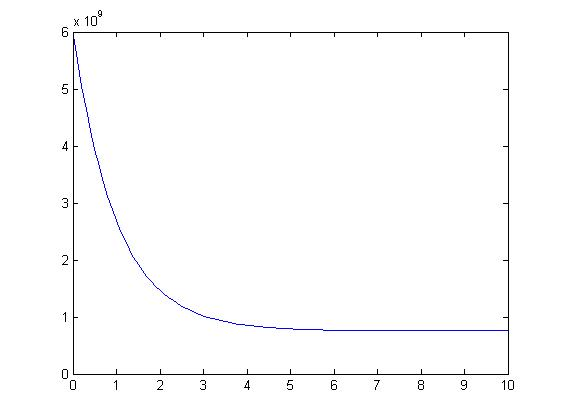
\includegraphics[scale=0.6]{./pic/duiliu.jpg}
\caption{对流方程的图像,数据取自巨大芽孢杆菌对流方程}\label{pic:duiliu_nnn}
\end{figure}
\subsection{对流扩散反应方程求解}
求解对流扩散反应方程是比较复杂的。现考虑采用线性变换的方法将一阶偏导数项消去,化成单纯的扩散方程再来解。\par
目前,本项工作正在进行。
\section{有限差分法求解数学模型}
考虑一个简单的对流扩散方程
\begin{equation}\label{equ:cf_dkfangc}
	\dfrac{\partial u}{\partial t}+a\dfrac{\partial u}{\partial x}=\nu\dfrac{\partial^2 u}{\partial x^2}
\end{equation}
其中a、$\nu$ 为常数,$\nu>0$,给定初值
\begin{equation}
	u(x,0)=g(x)
\end{equation}
构成了\textbf{对流扩散方程}的初值问题,在我们的模型中,它是一个对流占优的扩散问题。\par
将方程~\ref{equ:cf_dkfangc}~差分,有
\begin{equation}\label{equ:cf_dkfangct}
	\dfrac{u^{n+1}_j-u^{n}_{j}}{\tau}+a\dfrac{u^{n}_{j+1}-u^n_{j-1}}{2h}=\nu\dfrac{u^n_{j+1}-2u^n_j+u^n_{j-1}}{h^2}
\end{equation}
其截断误差为$O(\tau+h^2)$。\par
下面来分析差分格式~\ref{equ:cf_dkfangct}~的稳定性,令
\begin{equation}
	\lambda = a\dfrac{\tau}{h},\quad\mu=\nu\dfrac{\tau}{h^2}
\end{equation}
则差分格式~\ref{equ:cf_dkfangct}~改写为
\begin{equation}\label{equ:cf_dkmmm}
u^{n+1}_j=u^n_j-\frac{1}{2}\lambda(u^n_{j+1}-u^n_{j-1})+\mu(u^n_{j+1}-2u^n_j+u^n_{j-1})
\end{equation}\par
我们给出用于判断差分格式稳定性的\textbf{von Neumann}~定理,即
\begin{Theorem}[von Neumann定理]
差分格式
\begin{equation}
	u^{n+1}_j=C(x_j,\tau)u^n_j
\end{equation}
稳定的必要条件是当$\tau\leq\tau_0$,$n\tau\leq T$,对所有的k有
\begin{equation}
	\left|\lambda_j(G(\tau,k))\right| \leq 1+M\tau,\quad j=1,2,\cdots,p,
\end{equation}
其中$\left|\lambda_j(G(\tau,k))\right|$表示$G(\tau,k)$的特征值,$M$为常数。
\end{Theorem}\par
式~\ref{equ:cf_dkmmm}~的增长因子为
\begin{equation}
	G(\tau,k)=1-2\mu(1-\cos kh)-i\lambda\sin kh
\end{equation}
模的平方为
\begin{equation}
\begin{aligned}
	|G(\tau,k)|^2 &= [1-2\mu(1-\cos kh)]^2+\lambda^2\sin^2 kh\\
				  &= 1-4\mu(1-\cos kh)+4\mu^2(1-\cos kh)^2+\lambda^2\sin^2 kh\\
				  &= 1-(1-\cos kh)[4\mu-4\mu^2(1-\cos kh)-\lambda^2(1+\cos kh)]
\end{aligned}				  
\end{equation}
差分格式稳定的充分条件为
\begin{equation}
4\mu-4\mu^2(1-\cos kh)-\lambda^2(1+\cos kh) \geq 0
\end{equation}
即
\begin{equation}
(2\lambda^2-8\mu^2)\dfrac{1-\cos kh}{2}+4\mu-2\lambda^2 \geq 0
\end{equation}
注意到$\dfrac{1}{2}(1-\cos kh)\in[0,1]$,上式应满足
\begin{equation}
(2\lambda^2-8\mu^2)+4\mu-2\lambda^2 \geq 0,\quad 4\mu-2\lambda^2 \geq 0
\end{equation}
由此得到差分格式~\ref{equ:cf_dkfangct}~的稳定性限制为
\begin{equation}
\tau \leq \dfrac{2\nu}{a^2}
\end{equation}
\begin{equation}
\nu\dfrac{\tau}{h^2}=\dfrac{1}{2}
\end{equation}\par
目前工作进行到这里,下一阶段将对差分法求解模型做更加深入的研究。
\section{模型仿真计算的结果}
利用MATLAB PDETool工具箱,采用有限元法,求解模型,其结果如附图~\ref{pic:1}~、~\ref{pic:2}、~\ref{pic:3}~、~\ref{pic:4}~、~\ref{pic:5}~、~\ref{pic:6}~所示。\par
%\begin{figure}[t]
%	\ffigbox[\FBwidth]{{
%	\begin{subfloatrow}[3]
%	\ffigbox{\caption{t=10}}{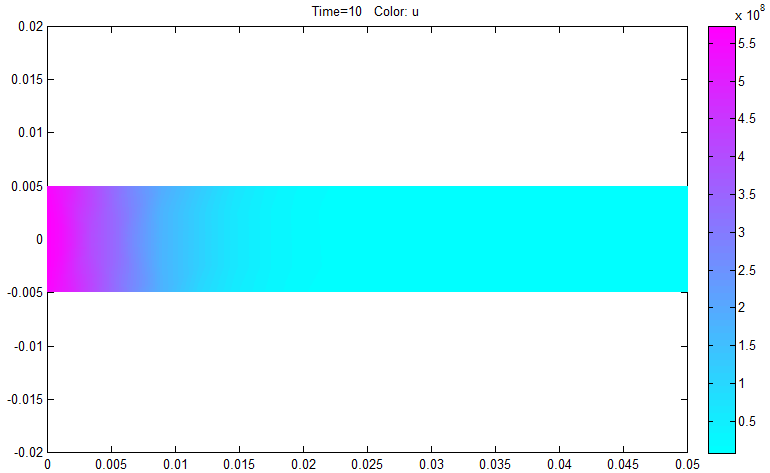
\includegraphics[scale=0.2]{./pic/01.png}}
%	\ffigbox{\caption{t=100}}{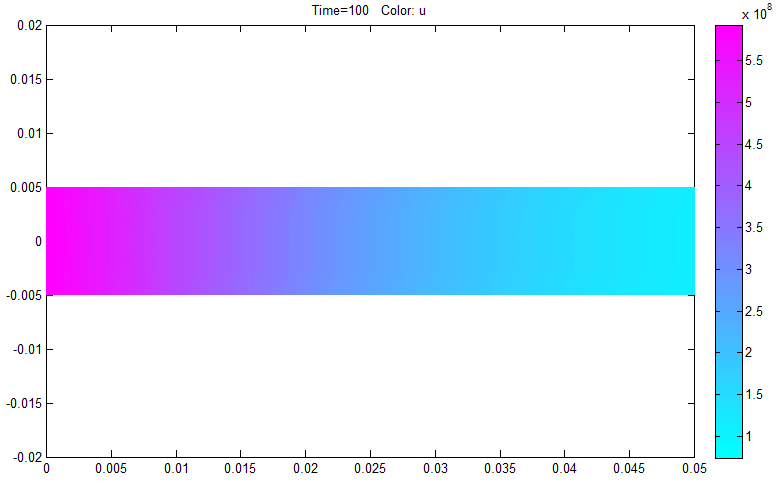
\includegraphics[scale=0.2]{./pic/01-100.png}}
%	\ffigbox{\caption{t=600}}{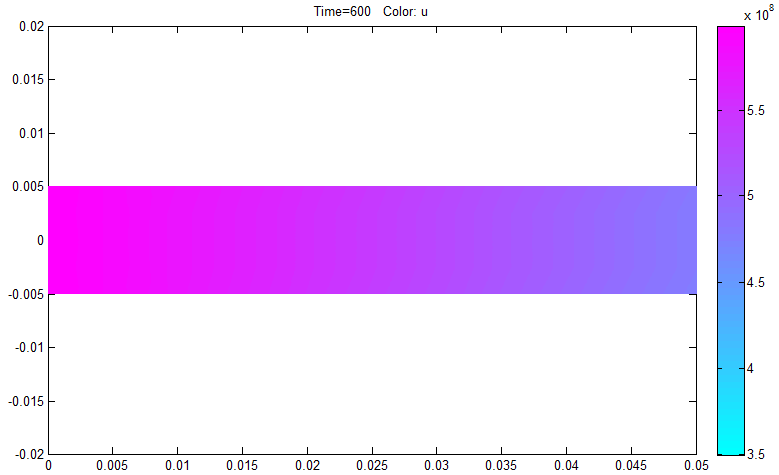
\includegraphics[scale=0.2]{./pic/01-600.png}}
%	\end{subfloatrow}}}{\caption{巨大芽孢杆菌}}
%	\ffigbox[\FBwidth]{{
%	\begin{subfloatrow}[3]
%	\ffigbox{\caption{t=10}}{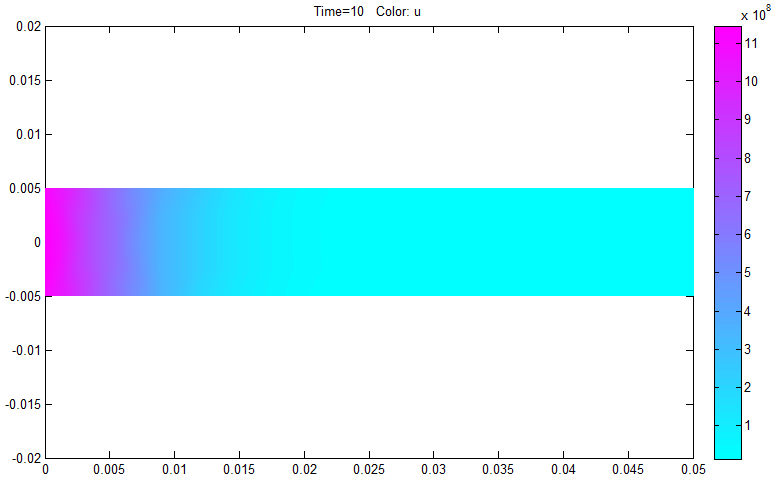
\includegraphics[scale=0.2]{./pic/02.png}}
%	\ffigbox{\caption{t=100}}{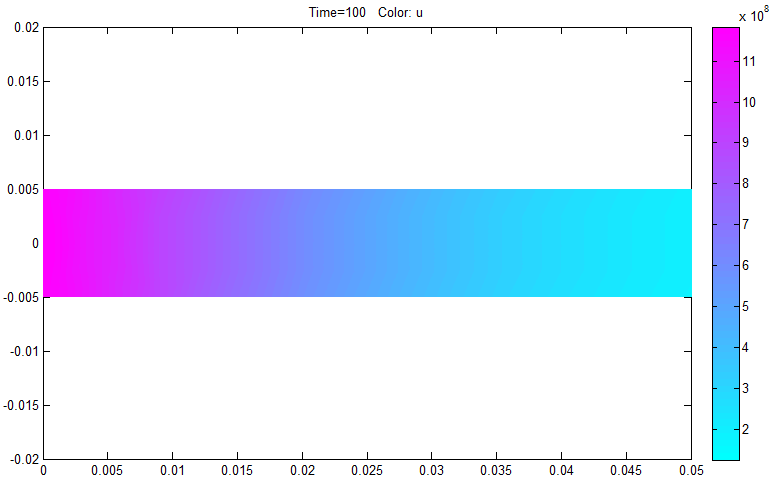
\includegraphics[scale=0.2]{./pic/02-100.png}}
%	\ffigbox{\caption{t=600}}{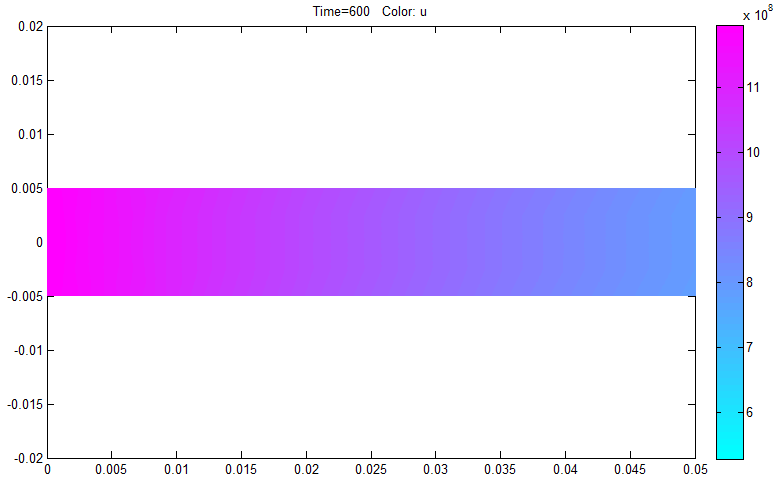
\includegraphics[scale=0.2]{./pic/02-600.png}}
%	\end{subfloatrow}}}{\caption{假单胞菌}}
%	\ffigbox[\FBwidth]{{
%	\begin{subfloatrow}[3]
%	\ffigbox{\caption{t=10}}{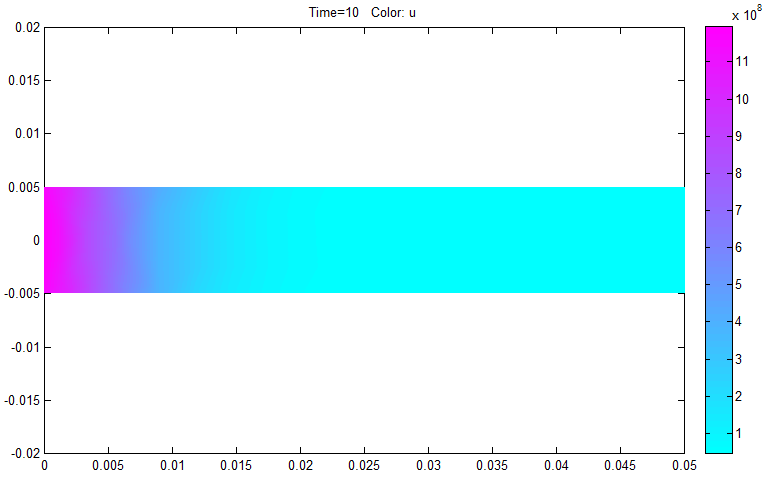
\includegraphics[scale=0.2]{./pic/03.png}}
%	\ffigbox{\caption{t=100}}{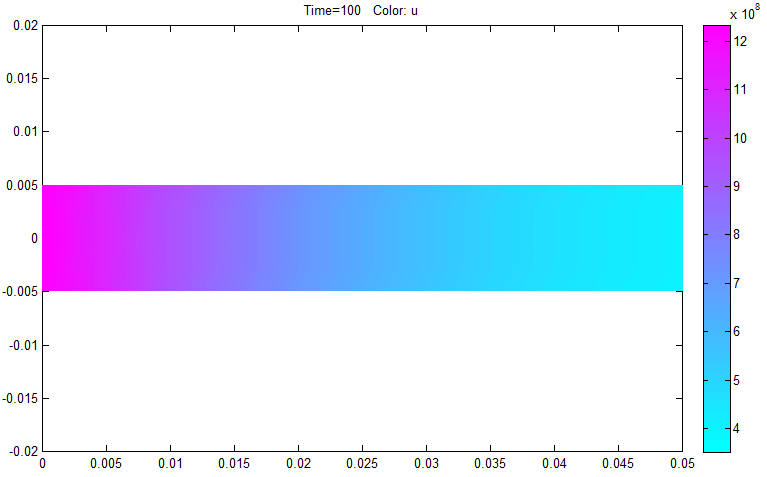
\includegraphics[scale=0.2]{./pic/03-100.png}}
%	\ffigbox{\caption{t=600}}{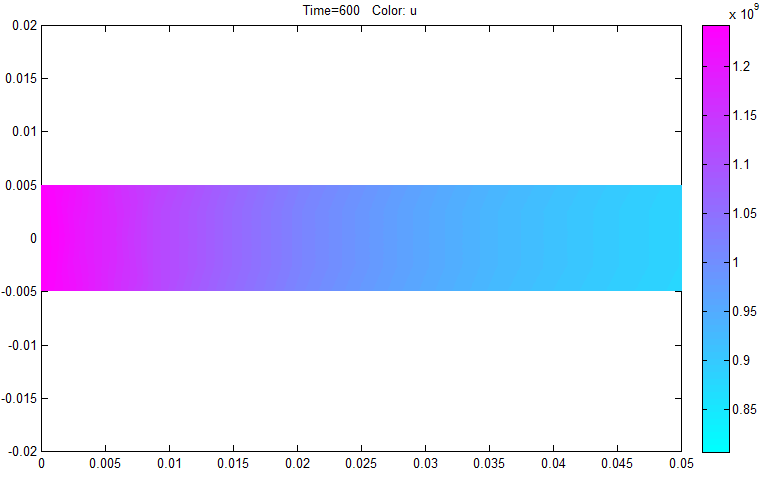
\includegraphics[scale=0.2]{./pic/03-600.png}}
%	\end{subfloatrow}}}{\caption{大肠杆菌}}
%	\ffigbox[\FBwidth]{{
%	\begin{subfloatrow}[3]
%	\ffigbox{\caption{t=10}}{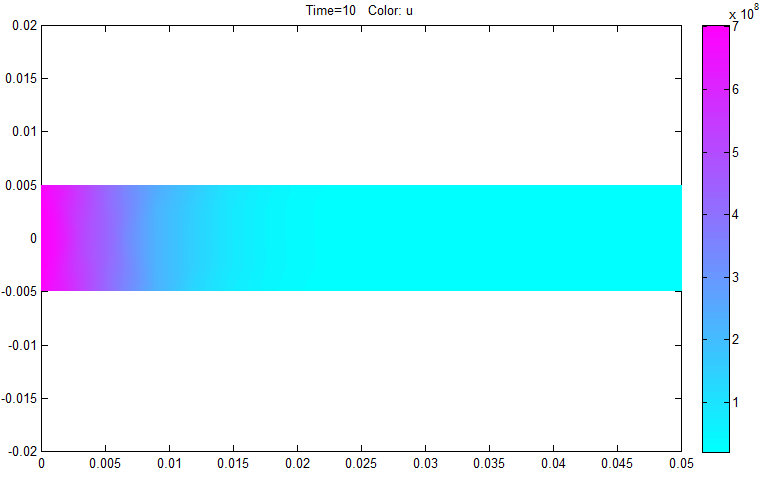
\includegraphics[scale=0.2]{./pic/04.png}}
%	\ffigbox{\caption{t=100}}{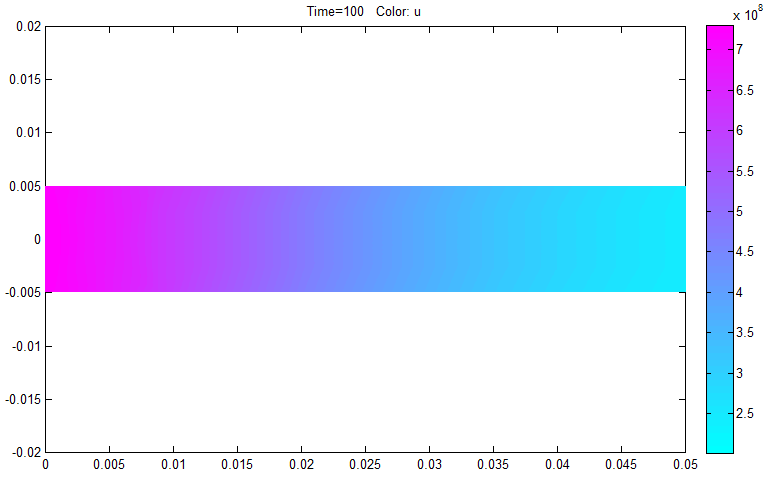
\includegraphics[scale=0.2]{./pic/04-100.png}}
%	\ffigbox{\caption{t=600}}{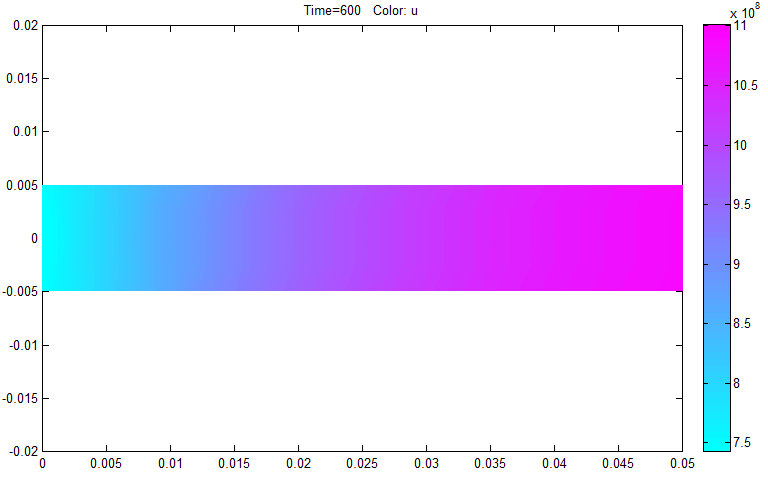
\includegraphics[scale=0.2]{./pic/04-600.png}}
%	\end{subfloatrow}}}{\caption{枯草芽孢杆菌}}
%	\ffigbox[\FBwidth]{{
%	\begin{subfloatrow}[3]
%	\ffigbox{\caption{t=10}}{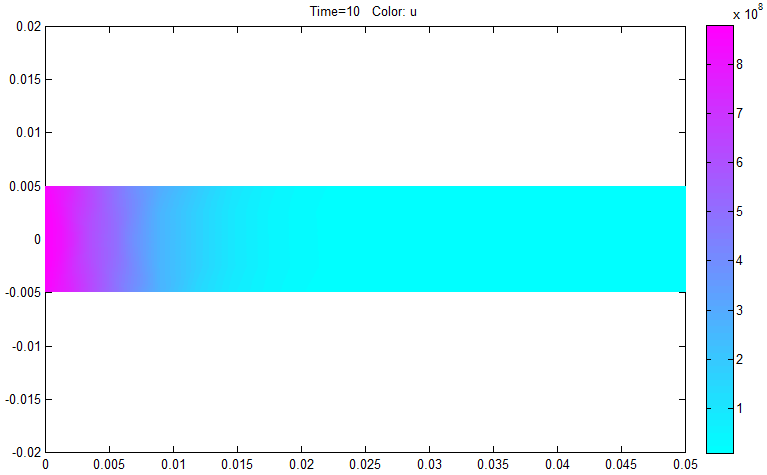
\includegraphics[scale=0.2]{./pic/05.png}}
%	\ffigbox{\caption{t=100}}{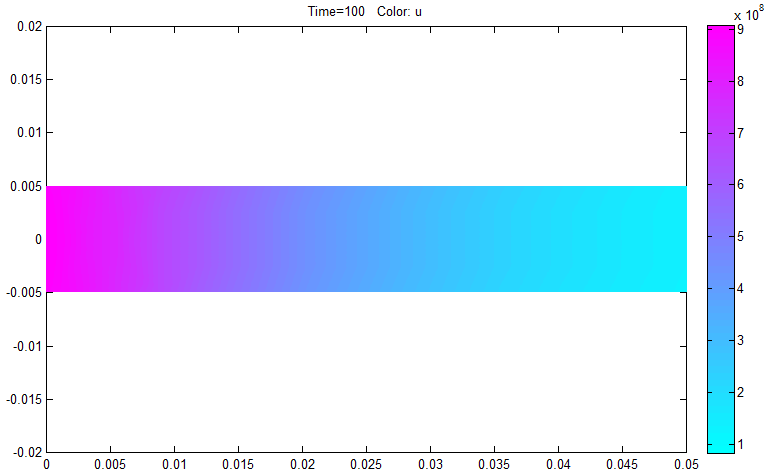
\includegraphics[scale=0.2]{./pic/05-100.png}}
%	\ffigbox{\caption{t=600}}{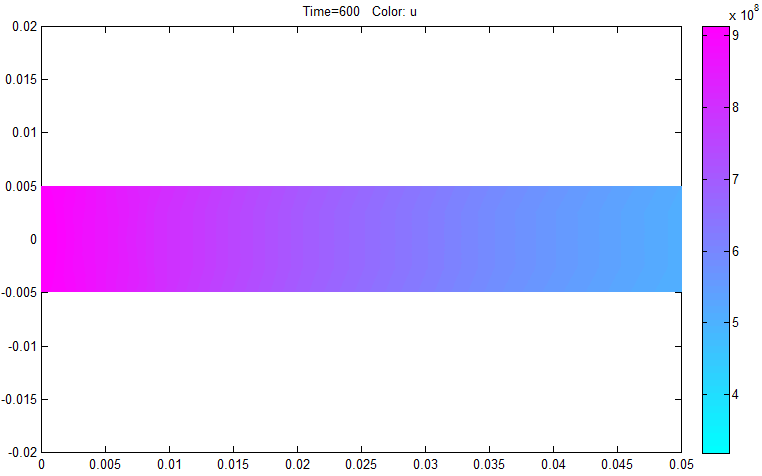
\includegraphics[scale=0.2]{./pic/05-600.png}}
%	\end{subfloatrow}}}{\caption{金黄色葡萄球菌}}
%	\ffigbox[\FBwidth]{{
%	\begin{subfloatrow}[3]
%	\ffigbox{\caption{t=10}}{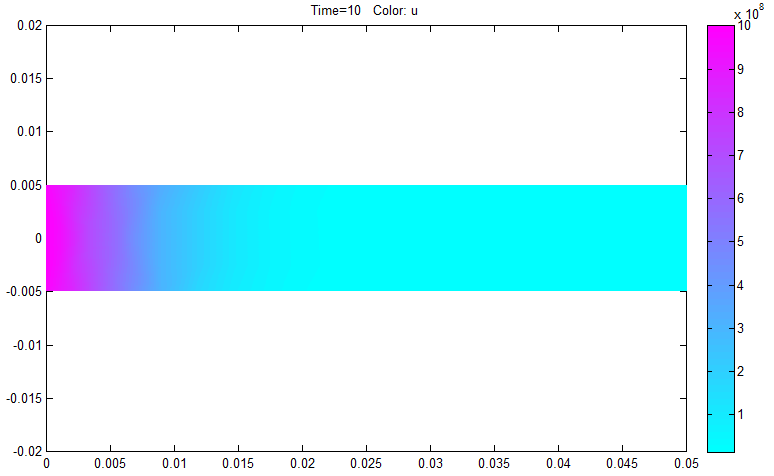
\includegraphics[scale=0.2]{./pic/06.png}}
%	\ffigbox{\caption{t=100}}{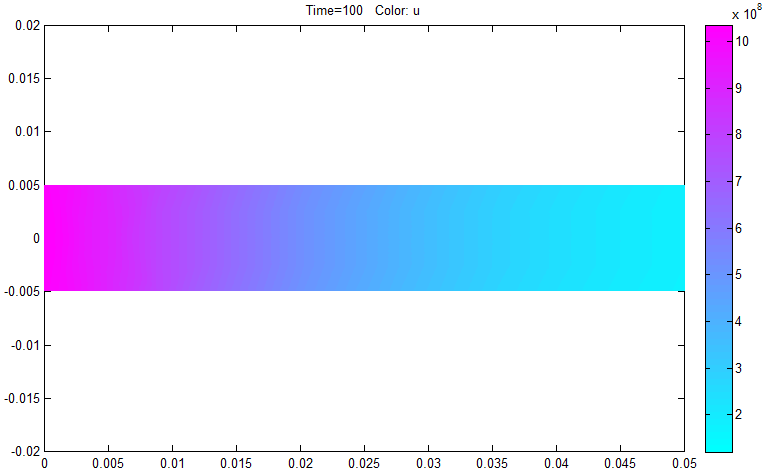
\includegraphics[scale=0.2]{./pic/06-100.png}}
%	\ffigbox{\caption{t=600}}{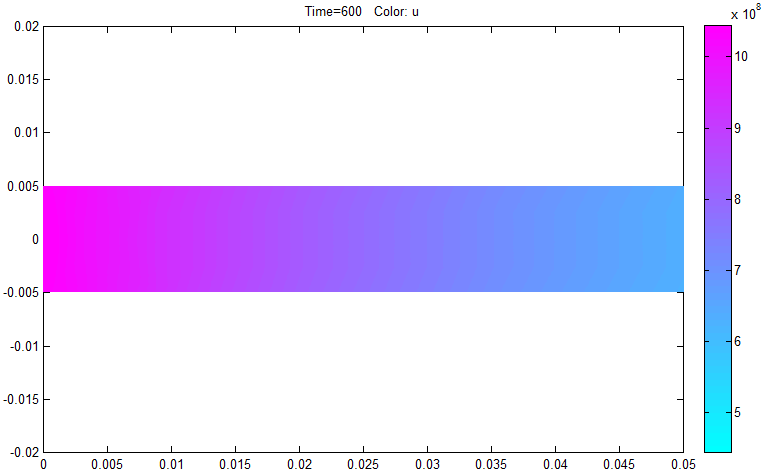
\includegraphics[scale=0.2]{./pic/06-600.png}}
%	\end{subfloatrow}}}{\caption{微球菌}}
%\end{figure}

%\begin{figure}[hp]
%\centering
%\subfloat[巨大芽孢杆菌]{\centering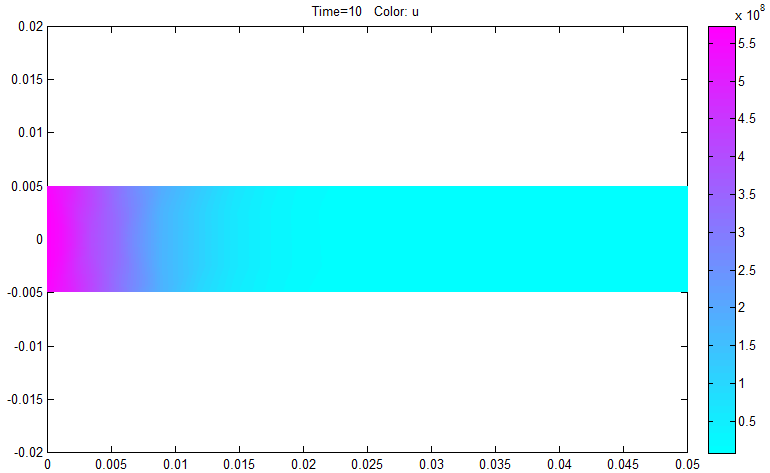
\includegraphics[scale=0.32]{./pic/01.png}}\hspace{10pt}
%\subfloat[假单胞菌]{\centering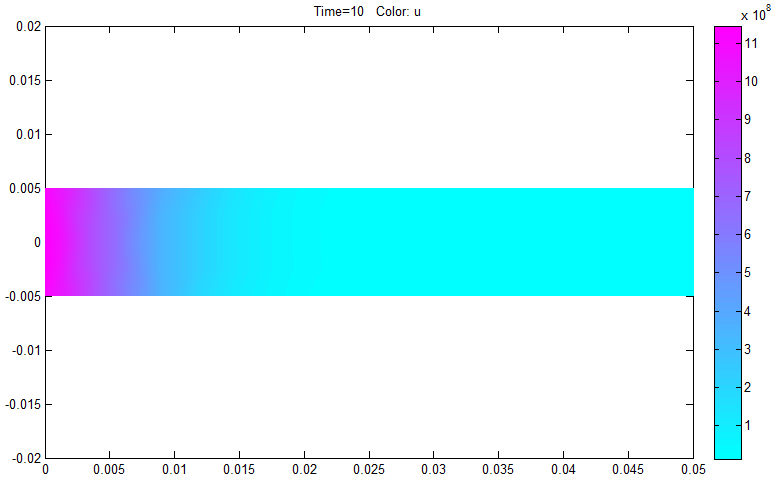
\includegraphics[scale=0.32]{./pic/02.png}}\\
%\subfloat[大肠杆菌]{\centering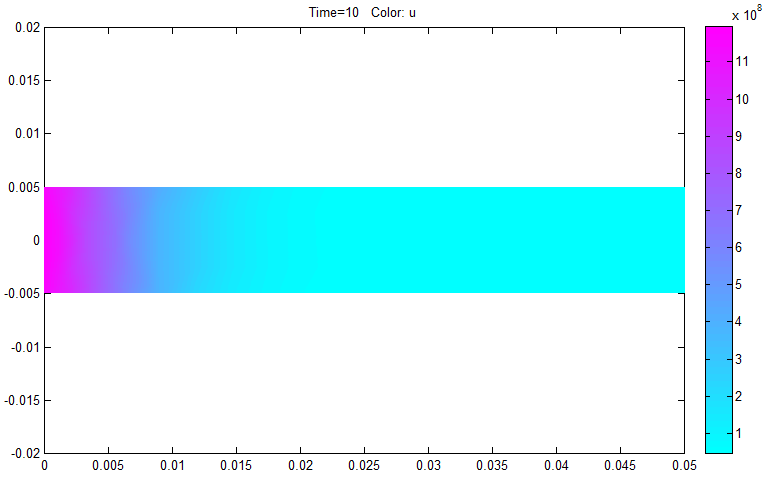
\includegraphics[scale=0.32]{./pic/03.png}}\hspace{10pt}
%\subfloat[枯草芽孢杆菌]{\centering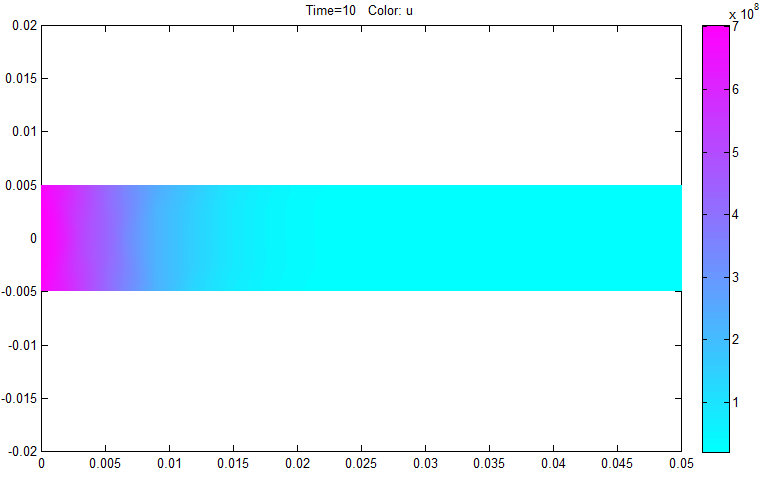
\includegraphics[scale=0.32]{./pic/04.png}}\\
%\subfloat[金黄色葡萄球菌]{\centering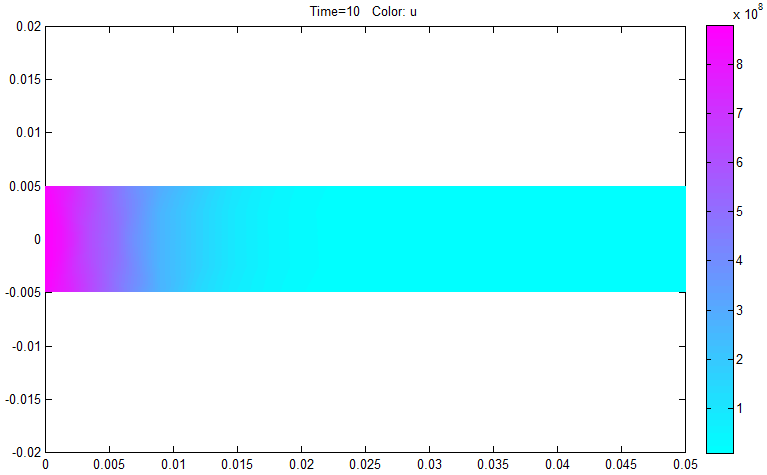
\includegraphics[scale=0.32]{./pic/05.png}}\hspace{10pt}
%\subfloat[微球菌]{\centering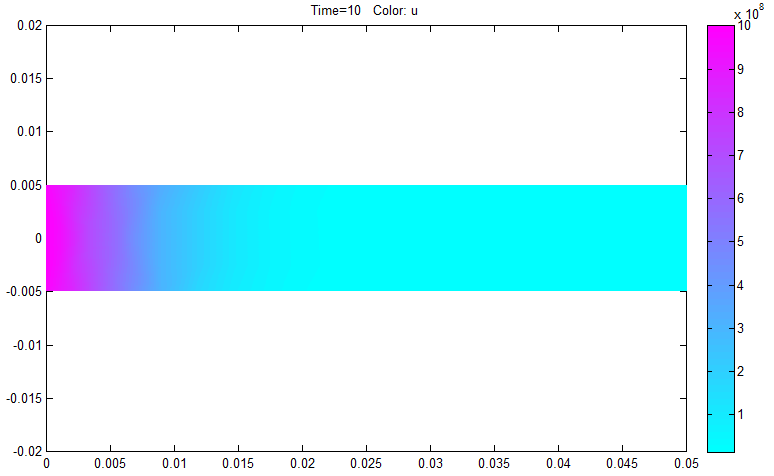
\includegraphics[scale=0.32]{./pic/06.png}}
%\caption{巨大芽孢杆菌等微生物运动模型仿真结果}\label{pic:xijun}
%\end{figure}
\section{接下来的工作计划}
接下来的主要工作在差分算法的研究与实现,尤其是三维模型的数值算法。如表~\ref{tab:test}~所示。
\begin{table}[htbp]
\centering\caption{\label{tab:test}工作计划表}
\begin{tabularx}{14cm}{cXc}
\toprule
时间 & \centering 工作内容 & 工作地点 \\
\midrule
2013年4月					& 三维方程求解算法的研究				&	机房			  \\
2013年5月					& 数值仿真程序的编制				&	机房			  \\
2013年6月					& 完成论文						&   实验室		  \\
\bottomrule
\end{tabularx}
\end{table}
\newpage
\nocite{*}
\bibliographystyle{ref/chinesebst}
\bibliography{ref/init}
\newpage
\section*{PDE工具箱求解程序}
\begin{verbatim}
function pdemodel
[pde_fig,ax]=pdeinit;
pdetool('appl_cb',1);
set(ax,'DataAspectRatio',[1 0.0060000000000000001 1]);
set(ax,'PlotBoxAspectRatio',[250 166.66666666666666 50]);
set(ax,'XLim',[0 10]);
set(ax,'YLim',[-0.02 0.02]);
set(ax,'XTickMode','auto');
set(ax,'YTickMode','auto');

% Geometry description:
pderect([0 10 0.0050000000000000001 -0.0050000000000000001],'R1');
set(findobj(get(pde_fig,'Children'),'Tag','PDEEval'),'String','R1')

% Boundary conditions:
pdetool('changemode',0)
pdesetbd(4,...
'dir',...
1,...
'1',...
'6e8')
pdesetbd(3,...
'neu',...
1,...
'0',...
'0')
pdesetbd(2,...
'neu',...
1,...
'0',...
'0')
pdesetbd(1,...
'neu',...
1,...
'0',...
'0')

% Mesh generation:
setappdata(pde_fig,'Hgrad',1.3);
setappdata(pde_fig,'refinemethod','regular');
setappdata(pde_fig,'jiggle',char('on','mean',''));
pdetool('initmesh')
pdetool('refine')
pdetool('refine')

% PDE coefficients:
pdeseteq(2,...
'3.66e-6',...
'1.035e-3',...
'7.819e5',...
'1.0',...
'0:10',...
'0.0',...
'0.0',...
'[0 100]')
setappdata(pde_fig,'currparam',...
['3.66e-6 ';...
'1.035e-3';...
'7.819e5 ';...
'1.0     '])

% Solve parameters:
setappdata(pde_fig,'solveparam',...
str2mat('0','2016','10','pdeadworst',...
'0.5','longest','0','1E-4','','fixed','Inf'))

% Plotflags and user data strings:
setappdata(pde_fig,'plotflags',[1 1 1 1 1 1 1 1 0 0 0 11 1 0 0 0 0 1]);
setappdata(pde_fig,'colstring','');
setappdata(pde_fig,'arrowstring','');
setappdata(pde_fig,'deformstring','');
setappdata(pde_fig,'heightstring','');

% Solve PDE:
pdetool('solve')
\end{verbatim}
\newpage
\section*{附图(仿真结果)}
\begin{figure}[h]
\subfloat[$t=10$]{\centering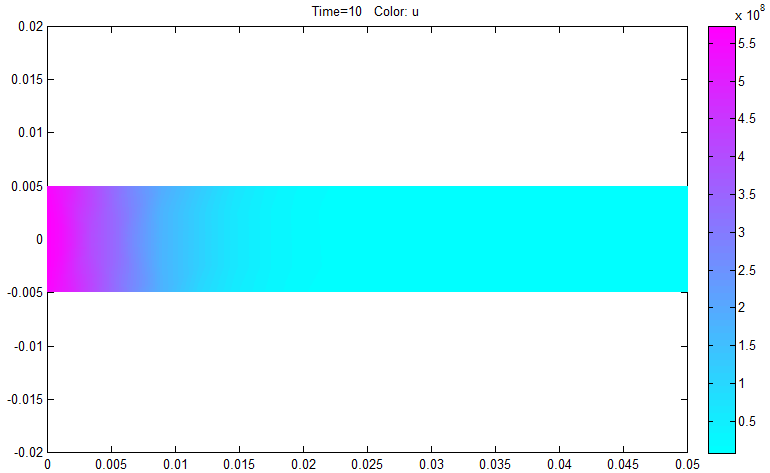
\includegraphics[scale=0.2]{./pic/01.png}}\hspace{10pt}
\subfloat[$t=100$]{\centering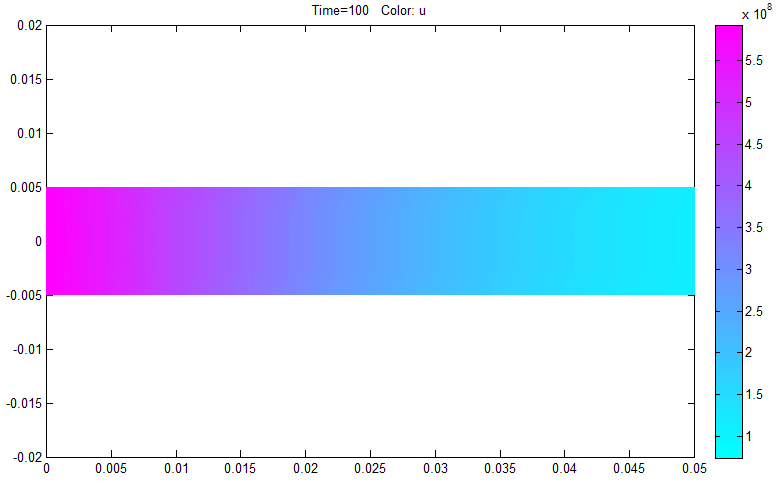
\includegraphics[scale=0.2]{./pic/01-100.png}}\hspace{10pt}
\subfloat[$t=600$]{\centering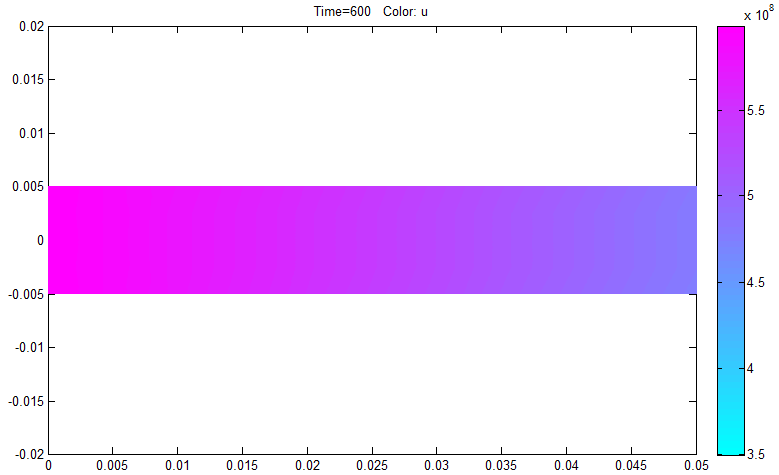
\includegraphics[scale=0.2]{./pic/01-600.png}}\hspace{10pt}
\caption{巨大芽孢杆菌的仿真结果}\label{pic:1}
\end{figure}
\begin{figure}[h]
\centering
\subfloat[$t=10$]{\centering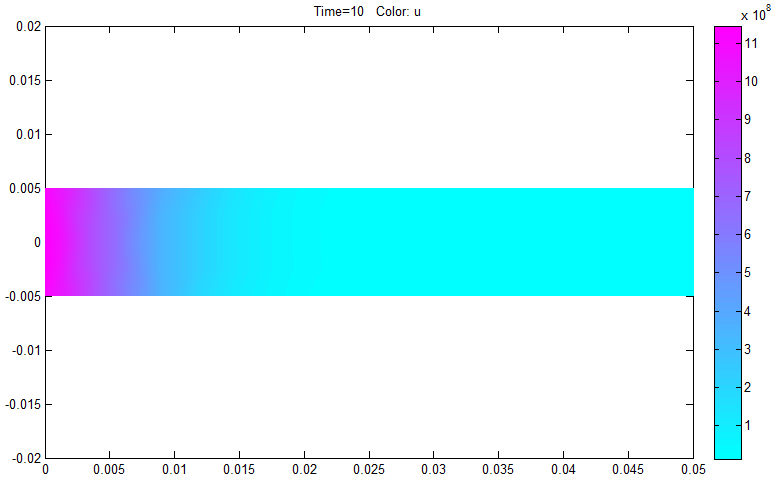
\includegraphics[scale=0.2]{./pic/02.png}}\hspace{10pt}
\subfloat[$t=100$]{\centering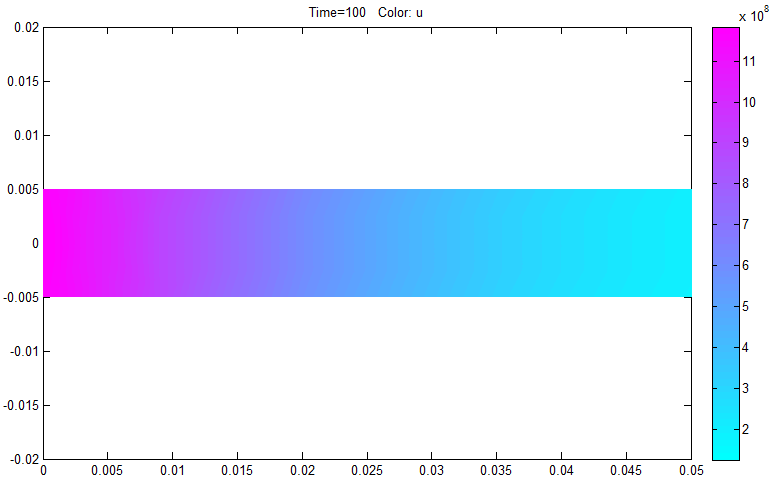
\includegraphics[scale=0.2]{./pic/02-100.png}}\hspace{10pt}
\subfloat[$t=600$]{\centering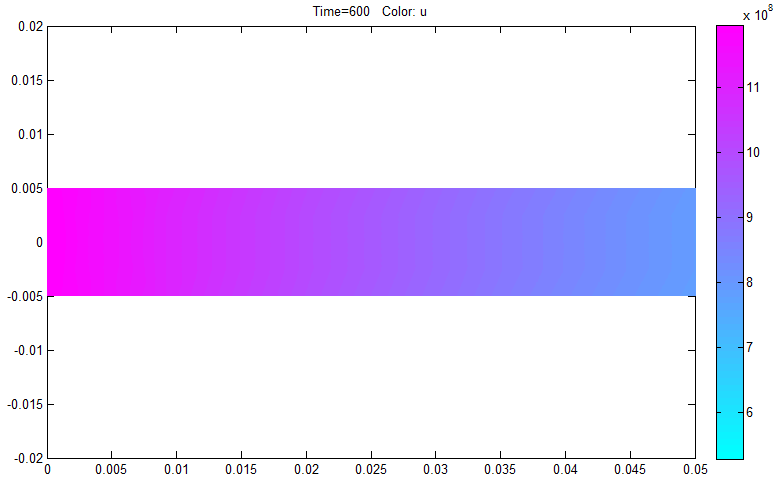
\includegraphics[scale=0.2]{./pic/02-600.png}}\hspace{10pt}
\caption{假单胞菌的仿真结果}\label{pic:2}
\end{figure}
\begin{figure}[h]
\centering
\subfloat[$t=10$]{\centering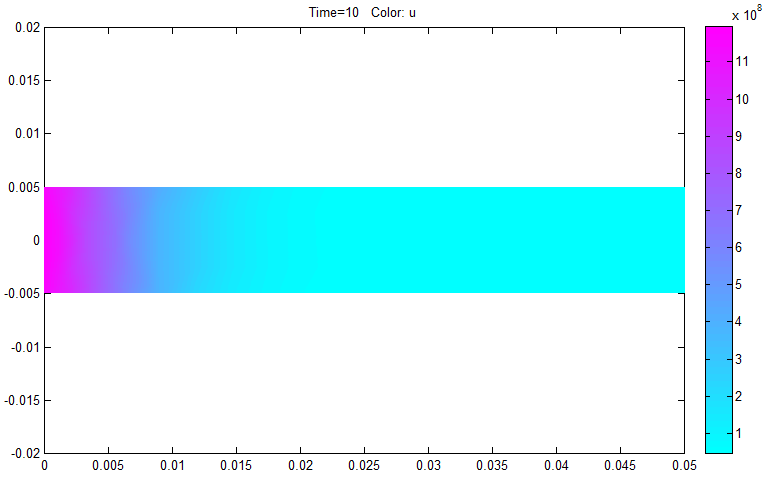
\includegraphics[scale=0.2]{./pic/03.png}}\hspace{10pt}
\subfloat[$t=100$]{\centering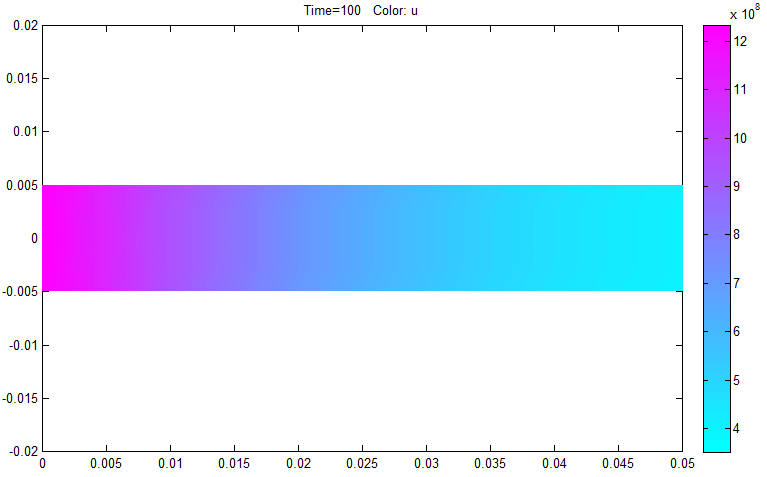
\includegraphics[scale=0.2]{./pic/03-100.png}}\hspace{10pt}
\subfloat[$t=600$]{\centering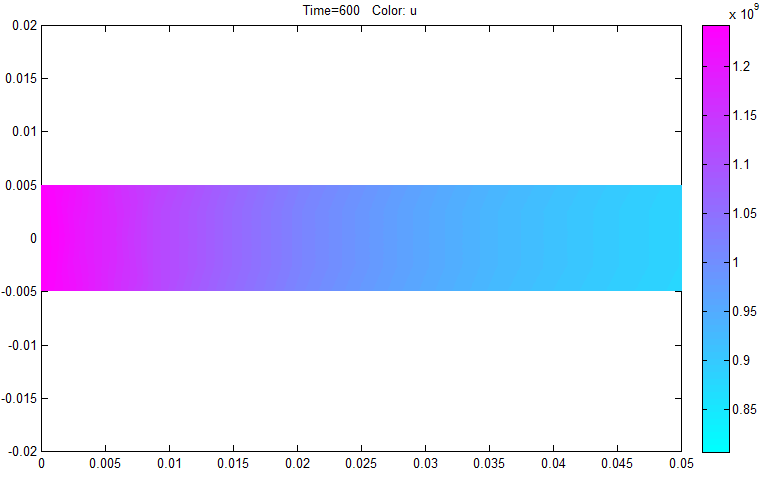
\includegraphics[scale=0.2]{./pic/03-600.png}}\hspace{10pt}
\caption{大肠杆菌的仿真结果}\label{pic:3}
\end{figure}
\begin{figure}[h]
\centering
\subfloat[$t=10$]{\centering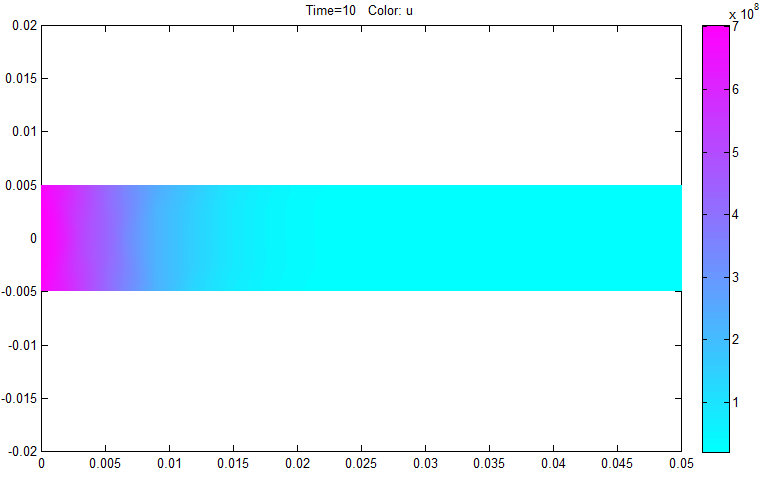
\includegraphics[scale=0.2]{./pic/04.png}}\hspace{10pt}
\subfloat[$t=100$]{\centering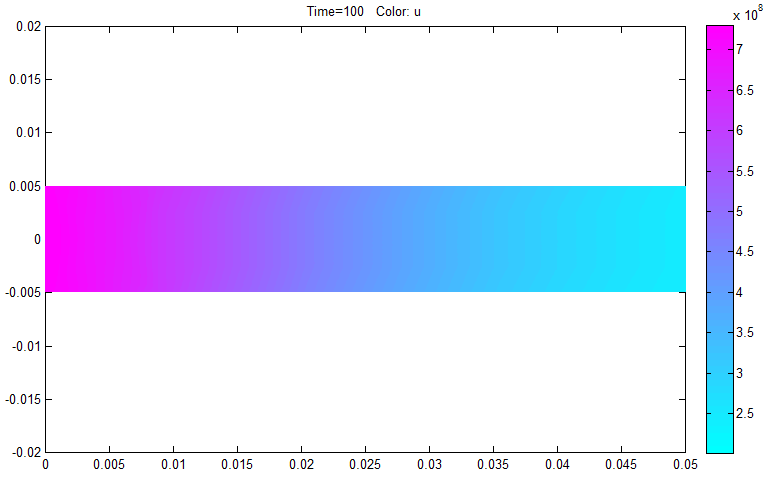
\includegraphics[scale=0.2]{./pic/04-100.png}}\hspace{10pt}
\subfloat[$t=600$]{\centering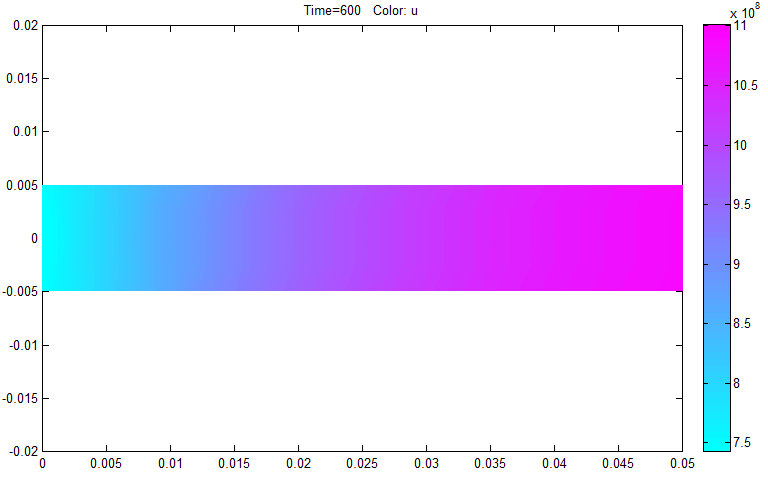
\includegraphics[scale=0.2]{./pic/04-600.png}}\hspace{10pt}
\caption{枯草芽孢杆菌的仿真结果}\label{pic:4}
\end{figure}
\begin{figure}[h]
\centering
\subfloat[$t=10$]{\centering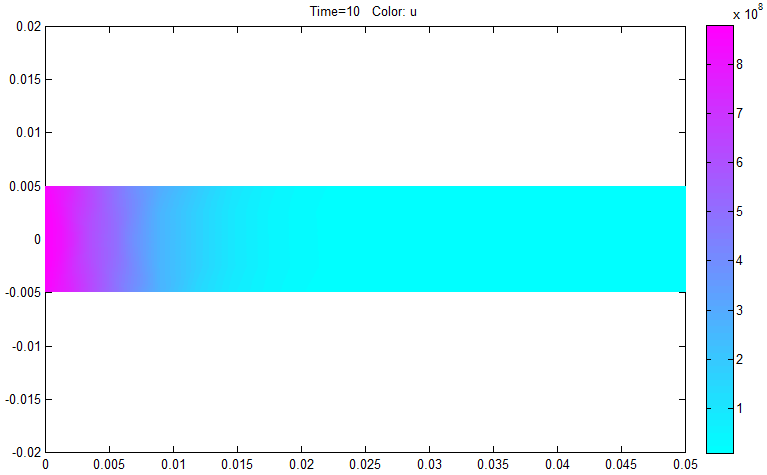
\includegraphics[scale=0.2]{./pic/05.png}}\hspace{10pt}
\subfloat[$t=100$]{\centering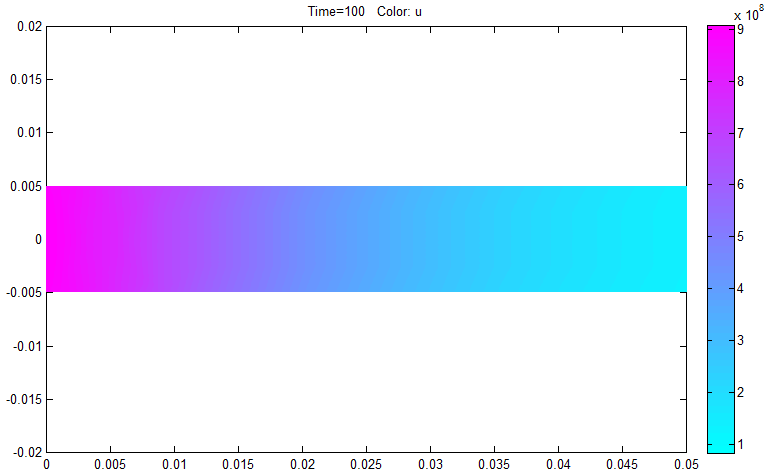
\includegraphics[scale=0.2]{./pic/05-100.png}}\hspace{10pt}
\subfloat[$t=600$]{\centering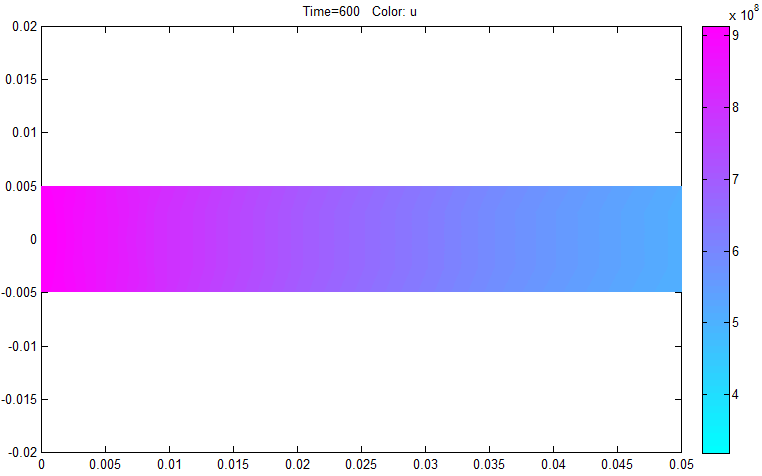
\includegraphics[scale=0.2]{./pic/05-600.png}}\hspace{10pt}
\caption{金黄色葡萄球菌的仿真结果}\label{pic:5}
\end{figure}
\begin{figure}[h]
\centering
\subfloat[$t=10$]{\centering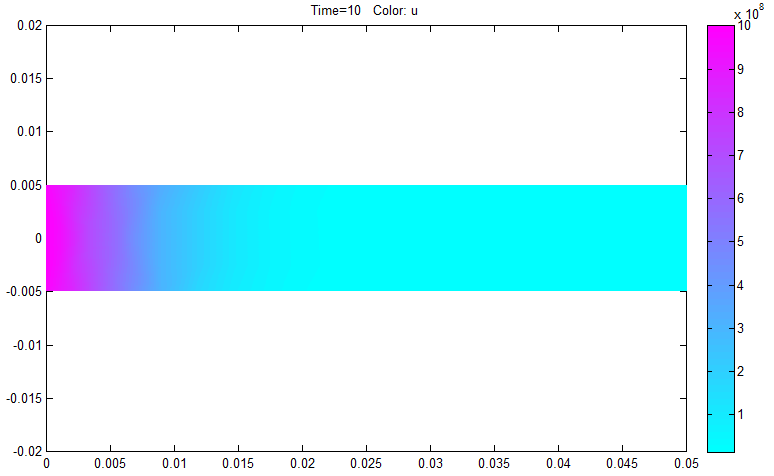
\includegraphics[scale=0.2]{./pic/06.png}}\hspace{10pt}
\subfloat[$t=100$]{\centering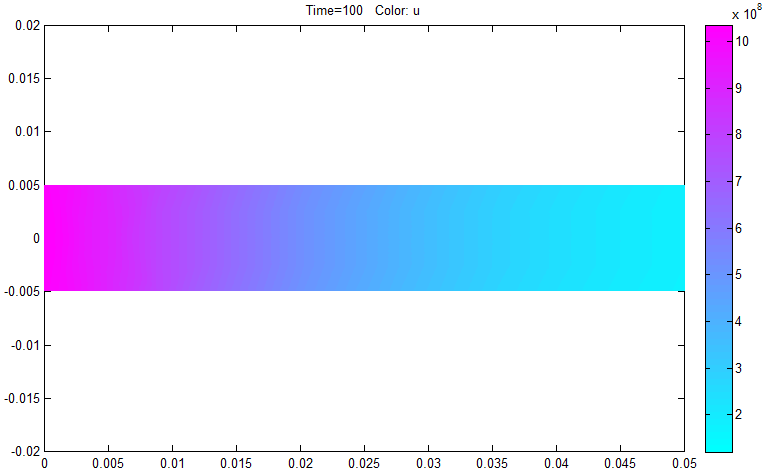
\includegraphics[scale=0.2]{./pic/06-100.png}}\hspace{10pt}
\subfloat[$t=600$]{\centering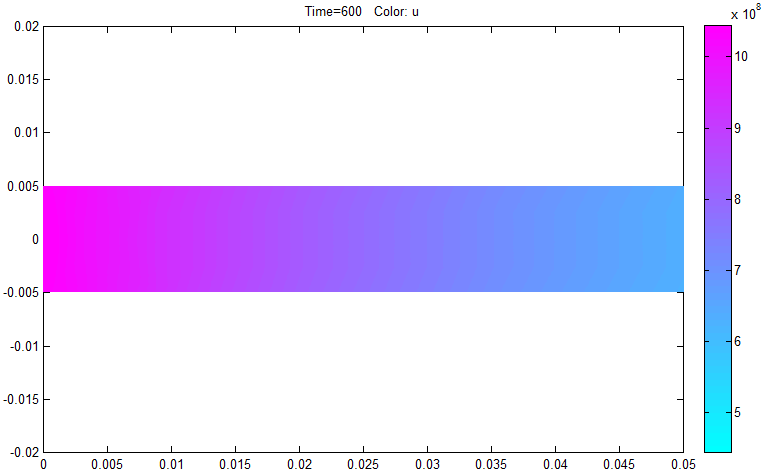
\includegraphics[scale=0.2]{./pic/06-600.png}}\hspace{10pt}
\caption{微球菌的仿真结果}\label{pic:6}
\end{figure}

\end{document}
